%課題研究レジュメテンプレート ver. 1.2

\documentclass[uplatex]{jsarticle}
\usepackage[top=20mm,bottom=20mm,left=20mm,right=20mm]{geometry}
\usepackage[T1]{fontenc}
\usepackage{txfonts}
\usepackage{wrapfig}
\usepackage[expert,deluxe]{otf}
\usepackage[dvipdfmx,hiresbb]{graphicx}
\usepackage[dvipdfmx]{hyperref}
\usepackage{pxjahyper}
\usepackage{secdot}

\makeatletter
  \renewcommand{\section}{%
    \if@slide\clearpage\fi
    \@startsection{section}{1}{\z@}%
    {\Cvs \@plus.5\Cdp \@minus.2\Cdp}% 前アキ
    {.5\Cvs \@plus.3\Cdp}% 後アキ
    %{\normalfont\Large\headfont\raggedright}}
    {\normalfont\raggedright}}

  \renewcommand{\subsection}{\@startsection{subsection}{2}{\z@}%
    {\Cvs \@plus.5\Cdp \@minus.2\Cdp}% 前アキ
    {.5\Cvs \@plus.3\Cdp}% 後アキ
    %{\normalfont\large\headfont}}
    {\normalfont}}

  \renewcommand{\subsubsection}{\@startsection{subsubsection}{3}{\z@}%
    {\Cvs \@plus.5\Cdp \@minus.2\Cdp}%
    {\z@}%
    %{\normalfont\normalsize\headfont}}
    {\normalfont}}
\makeatother
%ここから上を編集する必要はない.





\title{\vspace{-14mm}MBTIを用いた早期リスク特定}
\author{PMコース 矢吹研究室 1442085 中村真悟}
\date{}%日付を入れる必要はない.
\pagestyle{empty}%ページ番号は振らない.
\begin{document}
\maketitle


{研究の背景}

プロジェクトマネジメントとはヒト・モノ・カネ・資源を管理することである.この中で最もプロジェクトに関わり,かつ対処が確立しにくいのはヒトであると私は考える.

プロジェクトマネジメントにおいて,メンバとは必ず顔見知りになるということはない.今マネジメントしているプロジェクトのメンバはどのような人なのか.すぐにわかるわけではない.どのようにしたら改善できるのだろうか.

チームメンバを固定してしまうことである.当然そうすることができれば苦労はしないだろうが,プロジェクトの定義上困難な話である.では,プロジェクトマネージャがより早くメンバのことを,人間的特徴を把握することができればどうだろうか.

ユングの類型論を発展させたMBTIというものがある.人の考え方を
\begin{itemize}
\item 内向:I・外向:E
\item 感覚:S・直感:N
\item 思考:T・感情:F
\item 判断的態度:J・知覚的態度:P
\end{itemize}
の4指標の組み合わせで16タイプに分類するものである.この技法はキャリアカウンセリングやリーダーシップ開発,チームビルディングなどに使われることが多い.

このMBTIを用いて,プロジェクトのメンバの大まかな性格を理解し,メンバの相互作用が原因となって起きる事象の予測を行うことはできないのだろうかと考える.
以上のことから本研究ではMBTIを用いて,プロジェクトを円滑に遂行する方法を研究する.




\section{研究の目的}

本研究の目的は,チームメンバのMBTIの16タイプの相互作用がプロジェクトにどのような影響をもたらしているのかを調べる.その結果から,一つ目にチームメンバの編成によるメンバ間のリスクを特定できるようにすることである.二つ目に,プロジェクトの早期段階から注視すべき発生確率の高いリスクを明確にすることである.






\section{プロジェクトマネジメントの関連}

本研究では,PMBOKにおけるリスク・マネジメントに関連する.MBTIは自己理解メソッドであり自己成長を促すため,人的資源マネジメントに関連づく.また,MBTIはチームビルディングに用いることができる.さらにはメンバ間の円滑なコミュニケーション向上が期待できるため,コミュニケーションマネジメントに関連しているといえる.

\section{研究方法}

以下の手順で研究を進める.
\begin{itemize}
\item ソフトウェアコースのPM実験を受講する学生に対し,MBTIの性格検査を行い,メンバのタイプを調査
\item 各チームに対し,アンケートを行い実際にどのような事象が起きたか調査
\item アンケートの結果と個人のタイプ・チームのメンバでどのような関連があるのかを考察
\end{itemize}


\section{進捗}

上記の手順で,PM実験のソフトウェアコースを受講していた学生38人にMBTI診断とアンケート調査を行った.MBTI診断の結果は表\ref{wariai}の通りである.今回診断した学生38人の中には3タイプがいなかった.下記の表は2×2集計表での相関関係を求めたものである.この表において,値pが値Zの5%を下回るのであれば,相関があるということになる.

思考(T)型:情緒(F)型と「話し合いの場では自分から進んで発言した」という質問(表\ref{ke1})では値Zの5%の棄却域にあたる0.04を出したため,相関があると言える.
同じように規範(J)型:柔軟(P)型と「情報共有は問題なくできていた」という質問(表\ref{ke2})でも同様に相関があると言える.


\begin{figure}[h]
   \begin{tabular}{c}

      % 1
      \begin{minipage}{0.33\hsize}
        \begin{center}
   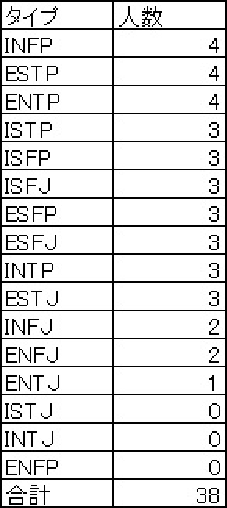
\includegraphics[width=3.5cm,clip]{wariai.pdf}
  \caption{MBTI結果}
  \label{wariai}
  \end{center}
 \end{minipage}

 \begin{minipage}{0.3\hsize}
   \begin{center}
  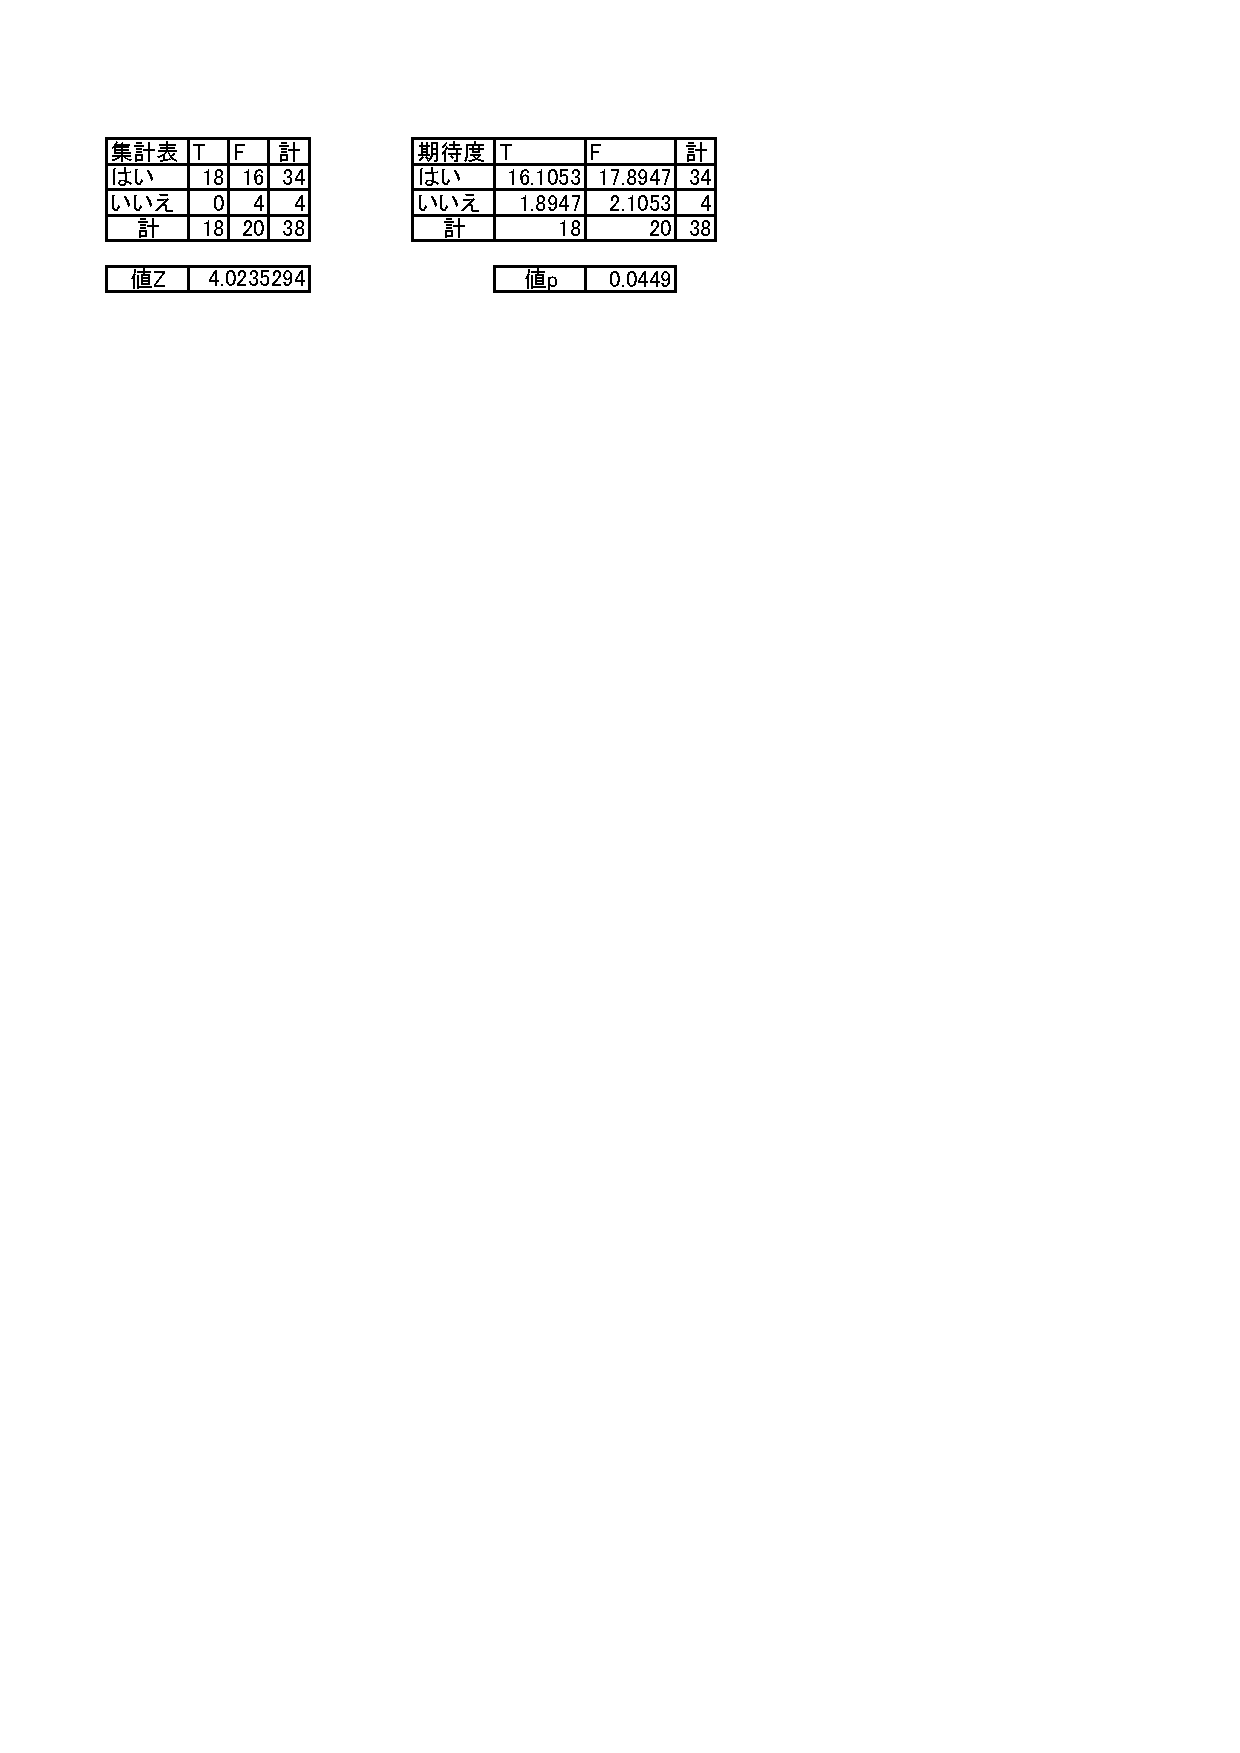
\includegraphics[width=9cm,clip]{kekka.pdf}
  \caption{T・Fと進んで発言したのクロス集計}
  \label{ke1}
   \end{center}
    \begin{center}  
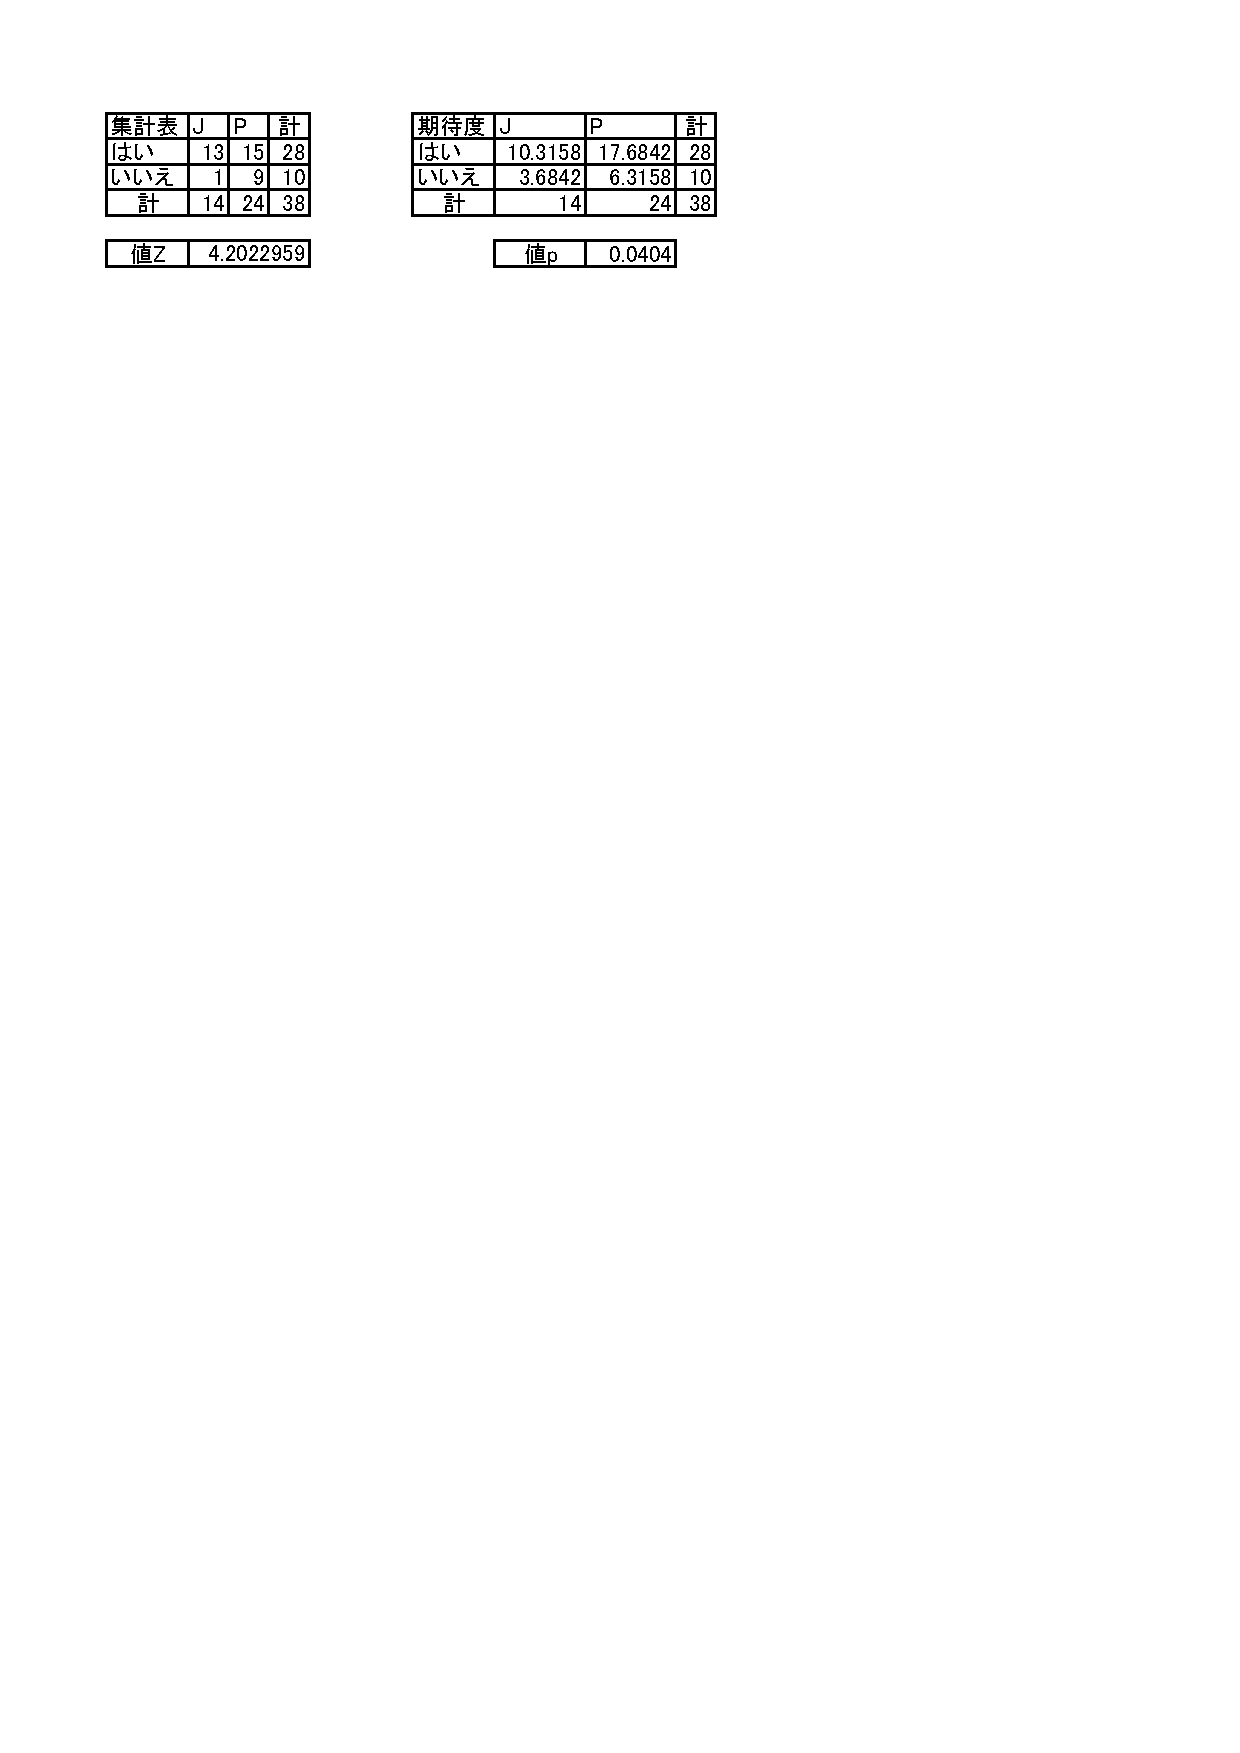
\includegraphics[width=9cm,clip]{kekka2.pdf}
  \caption{J・Pと情報共有は問題なくできていたのクロス集計}
  \label{ke2}
   \end{center}
 \end{minipage}
\end{tabular}
  \end{figure}


\section{今後の計画}
\begin{itemize}
\item 今回のアンケート結果を踏まえ,質を高める
\item PM実験後半組のデータを用いて仮説を立てる
\item 実証された相関が長期の場合どうなるのか,PM演習を受講する学生に対し同様の方法でアンケートを行い検証する
\end{itemize}




\nocite{BB19543658}\nocite{110003745117}\nocite{ylab2015}\nocite{katolab2015}\nocite{mbti}
\bibliographystyle{junsrt}
\bibliography{biblio}%「biblio.bib」というファイルが必要.

\end{document}
